\section{Heuristica de busqueda local}

Para encontrar soluciones aproximadas al problema de optimizar una funci\'on $f:S \rightarrow \mathbb{R}$ definida sobre un conjunto $S$ de instancias, la heur\'istica de b\'usqueda local consiste en tomar un elemento $e \in S$ y buscar entre los elementos ``cercanos'' a $e$ uno $e'$ en el cual el valor que toma la funci\'on sea mejor ($f(e') < f(e)$ \'o $f(e') > f(e)$ dependiendo de si se busca m\'inimo a o m\'aximo).
El concepto de cercan\'ia o vecidad se puede definir seg\'un cualquier criterio que se crea conveniente. Formalmente se puede ver como una relaci\'on $R \subseteq S \times S$, que es sim\'etrica y reflexiva. Se busca en lo posible que las vecindades de cada punto sean peque\~nas para que se pueda encontrar r\'apidamente un vecino mejor en caso de que exista.
La heur\'istica itera el procedimiento de optimizaci\'on local creando una sucesi\'on de soluciones aproximadas $(X_0, X_1, ... , X_m)$ en $S$ donde el elemento $X_m$ tiene la propiedad de ser un extremo local de la funci\'on $f$ seg\'un el criterio definido de vecindad.


\subsection{Criterio de vecindad}
Para el problema enunciado del TP, el conjunto $S$ es el conjunto de caminos entre el nodo de partida y el de llegada. Debido a que las $w_1$ y $w_2$ son funciones positivas, el camino acotado de costo m\'inimo estar\'a en $S' \subseteq S$, el subconjunto de todos los caminos simples. Por lo tanto solo se considerar\'a $S'$ como conjunto de instancias.
Se definir\'a primero la relaci\'on de vecindad. Ante todo, la notaci\'on ser\'a la siguiente. $C = (v_1, ..., v_m)$ ser\'a un camino y $A_c$ el conjunto de aristas que lo conforman. Dos caminos $C = (v_1, ... , v_n)$ y $C' = (v'_1, ... , v'_m)$ en $S'$ son vecinos $C \sim C'$ si se cumple alguna de las siguientes condiciones:

\begin{enumerate}
    \item $C = C'$
    \item $ \exists v \notin C \mid A_{c'} = A_c - \{(v_i,v_{i+1}),(v_{i+1},v_{i+2})\} + \{(v_i,v),(v,v_{i+2})\}$
    \item $ \exists v \notin C \mid A_{c'} = A_c - \{(v_i,v_{i+1})\} + \{(v_i,v),(v,v_{i+1})\}$
    \item $A_{c'} = A_c - \{(v_i,v_{i+1}), (v_{i+1},v_{i+2})\} + \{(v_i,v_{i+2})\}$

\end{enumerate}

\begin{figure}[H]
\centering
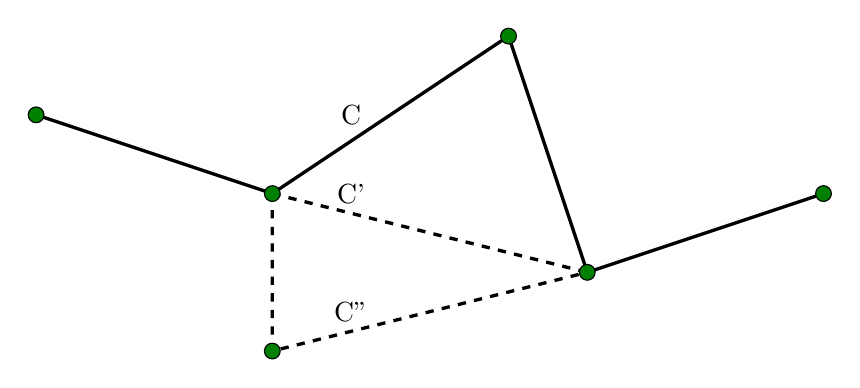
\begin{tikzpicture}

\draw[black, solid, very thick] (-1,2) -- (2,1) -- (5,3) -- (6,0) -- (9,1);
\draw[black, dashed, very thick] (2,1) -- (6,0);
\draw[black, dashed, very thick] (2,1) -- (2,-1)  -- (6,0);
\filldraw[fill=green!50!black, draw=black] (2,-1) circle [radius=1mm];
\filldraw[fill=green!50!black, draw=black] (-1,2) circle [radius=1mm];
\filldraw[fill=green!50!black, draw=black] (2,1) circle [radius=1mm];
\filldraw[fill=green!50!black, draw=black] (5,3) circle [radius=1mm];
\filldraw[fill=green!50!black, draw=black] (6,0) circle [radius=1mm];
\filldraw[fill=green!50!black, draw=black] (9,1) circle [radius=1mm];
\node(c) at (3,2) {C};
\node(c') at (3,1) {C'};
\node(c'') at (3,-0.5) {C''};

\end{tikzpicture}
\caption{Tres caminos vecinos entre si.}
\end{figure}

\subsection{Explicacion detallada del algoritmo propuesto}
Sea $s$ una solucion factible, es decir, un camino entre $u,v$ tal que el costo del camino $w_1 \leq K$,
para plantear esta heur\'istica definimos $N(s) = \{ $ conjunto de soluciones vecinas de s$\}$ = $\{$ caminos entre u,v tal que $w_1 \leq K$ y difieren en solo un nodo de $s\}$.\\

Se plantearon 3 posibles enfoques para aplicar busqueda local sobre esta vecindad, a continuacion se explicar\'an cada uno.

\subsubsection{Obtencion de la solucion inicial factible}

Para obtener la solucion inicial factible de nuestra heur\'istica ejecutamos el algoritmo de camino m\'inimo de Dijkstra, entre los nodos u y v, sobre la funcion $w_1$, acto seguido validamos si $dist(w_1, src, dst) > K$ entonces no existe soluci\'on factible, caso contrario tenemos una soluci\'on factible inicial para comenzar las 
iteraciones de busqueda local.

\subsubsection{Criterio de terminaci\'on}
El criterio de terminacion fue repetir las iteraciones sobre las nuevas soluciones que se iban obteniendo, hasta que no se obtiene mejora.
Siempre se aplica uno solo de los 3 metodos a las iteraciones, es decir, no se combinan.

\subsubsection{Pseudocodigo}

A continuaci\'on el pseudoc\'odigo de la b\'usqueda local.
\begin{algorithmic}

 \Procedure{$Bq\_Local$}{$Grafo\: g, \:vertice\: v_1,\: vertice \: v_2, \: int \: k, tipo\_busqueda$}{$\rightarrow lista<eje>\: camino$}

 \State $lista<eje> \: camino\: =\: dijkstra(g, \:v_1,\: v_2, \:costoW1)$
 \State  $bool\: hay\_mejora\: = \:true$

 \While{$hayMejora$}

  \State $switch(tipo\_busqueda)$
	\State$\: \: \: 	case\: subdividirPares$
		\State$\: \: \: \: \: 	\:hayMejora\: = \: bqLocalEntrePares(g,camino)$
	\State$	\: \: \: case\: contraerTriplas$		
		\State$\: \: \: \: \: 	\:hayMejora\: = \: bqLocalContraerTriplas(g,camino)$
	\State$	\: \: \: case \:mejorarTriplas:		$
		\State$\: \: \: \: \: 	\:hayMejora\: = \: bqlocalEntreTriplasReemplazando(g,camino)$

\EndWhile

 \State $return \:camino$

 \EndProcedure

\end{algorithmic}

\subsubsection{Reemplazar un nodo intermedio en una 3-upla consecutiva de nodos del camino}
Si el camino tiene longuitud 2, es decir hay una arista directa entre $u,v$ , no hay nada que hacer en este caso, caso contrario, sea $S = \{u,...,v_l, v_{l+1}, v_{l+2}, v_{l+3} ..., v\}$ la solucion actual. Lo que hace en este caso es iterar sobre todas las 3-uplas consecutivas del camino, en este ejemplo sea $(vl, v_{l+1}, v_{l+2})$ una 3-upla, $(v_{l+1}, v_{l+2}, v_{l+3})$ la siguiente a iterar, etc...\\ \\
Para cada 3-upla iterada se revisan los vecinos en comun entre los extremos de la 3-upla buscando una mejor conexi\'on entre extremos reemplazando el nodo intermedio 
como se indica en el grafico debajo, es decir, se busca una nueva conexion entre los extremos tal que, si el nuevo nodo intermedio es $v_t$, vale que:
\begin{itemize}
	\item Mejore la conexion de la 3-upla respecto a $w_2$, $w_2(vl, v_{t}) + w_2(vt, v_{l+2}) < w_2(vl, v_{l+1}) + w_2(v_{l+1}, v_{l+2})$
	\item Este cambio, reflejado en la nueva solucion candidata S', no sobrepase la cota K establecida sobre $w_1$, es decir, sea factible.
\end{itemize}


Una iteracion consiste en recorrer todas las 3-uplas del camino obteniendo de los vecinos en com\'un de los extremos de cada 3-upla, si es posible, la mejor forma de mejorar esta conexion, ademas recordando la mejor 3-upla para aplicar la mejora a lo largo de la iteraci\'on, tal que el camino resultante de aplicar esta mejora sea el minimo sobre $w_2$ en la vecindad $N(s)$. Mas formalmente, se busca una solucion vecina del camino S, tal que siendo $w_1(P), w_2(P)$ los costos sobre $w_1$ y $w_2$ respectivamente de una solucion, y $S' = S \setminus \{(v_k, v_{k+1}); (v_{k+1}, v_{k+2})\} \cup \{(v_k, v_t);(v_t, v_{k+2})\}$ la nueva solucion obtenida, entonces valga que:
\begin{itemize}
	\item Sea factible, pertenezca a $N(S)$, $ w_1(S') \leq K$
	\item Sea minima respecto de $w_2$ en la vecindad $N(S)$, $w_2(S') \leq w_2(T)$ $ \forall$ $ T \in N(S) $
\end{itemize}

\subsubsection{Insertar un nodo intermedio en un par consecutivo de nodos del camino}
Este enfoque es basicamente igual al anterior, solo que en lugar de iterar sobre 3-uplas reemplazando el nodo intermedio, se itera sobre pares consecutivos de nodos de la solucion S $(v_k, v_{k+1})$ buscando si existe, un vecino en comun entre los extremos tal que el sendero $(v_k, v_t, v_{k+1})$ tenga costo menor(de forma minima entre los vecinos) sobre $w_2$ que la arista directa y que reflejado en la solucion candidata S' que surge de aplicar este cambio, siga siengo factible($w_2(S') \leq K$). La iteracion de sigue siendo sobre toda la vecindad $N(S)$ y quedandose con el mejor $S' \in N(S)$ posible.


\subsubsection{Contracci\'on de 3-uplas}

Similar a los casos anteriores, itera sobre las 3-uplas de nodos del camino, intentando eliminar el nodo intermedio y buscar una arista que conecte directamente los nodos de los extremos. Sean los 3 nodos $v_1$, $v_2$ y $v_3$, y el subcamino de aristas formado por ellos $[ (v_1, v_2), (v_2, v_3)]$, se encontrar la arista $(v_1, v_3)$, tal que:

\begin{itemize}
	\item $costoW2((v_1, v_3)) \leq costoW2((v_1, v_2)) + costoW2((v_2, v_3))$
	\item Que el camino, eliminando el nodo $v_2$ y las aristass $(v_1, v_2), (v_2, v_3)$ y conectando los nodos $v_1$ y $v_3$ mediante la arista directa $(v_1, v_3)$ siga sin sobrepasar la cota K establecida sobre $w_1$, es decir, sea factible.
\end{itemize}

\subsection{Nivel de optimalidad de las soluciones}

La heur\'istica va a fallar en todos los casos en los cuales no se pueda mejorar un par o tripla de nodos agregando, quitando o reemplazando de a un nodo, por ejemplo, casos en los que la mejora sea un subcamino de longitud mayor a 2, o casos en los que el camino \'optimo no tiene ning\'in tipo de conexi\'on con el camino m\'inimo seg\'un $w_1$.

\subsubsection{Complejidad}

Podemos acotar la iteraci\'on sobre el camino con la mayor cantidad de nodos posibles que puede tener, es decir, $O(n)$. Por cada iteraci\'on, en cualquiera de los tres m\'etodos, se llama a la funci\'on $vecinos$ de dos nodos, lo cual est\'a acotado tambi\'en por $2*O(n)$. Por lo tanto, una iteraci\'on de b\'usqueda local tiene una complejidad de $O(n^2)$. La complejidad total de la heur\'istica no puede acotarse, ya que depende del criterio de terminaci\'on.

\subsection{Taboo list}
  Definimos una taboo list como una lista en la cual se encuentran los nodos que pertenecen al camino soluci\'on actual, de forma de evitar que la b\'usqueda local intente mejorar las conexiones utilizano nodos que ya pertenecen al camino.Esto es indispesable para evitar la generacion de ciclos en el caso de agregar un nodo al subdividir una arista o reemplazar un nodo
intermedio entre otros dos. Si se mantienen disjuntos disjuntos el conjunto de nodos del camino actual y los nodos restantes del grafo, cualquier eleccion que hagamos no generar\''a ciclos.

\vspace{2mm}

La taboo list est\'a implementada como un vector de bool que forma parte de los atributos de un camino del grafo, de forma de poder consultar la pertenencia de un nodo al camino en tiempo constante.

\vspace{2mm}

	Otra opcion considerada fue no restringir la b\'usqueda de nuevos nodos, pero luego deber\'ia realizarse una poda de ciclos del camino. En la muchos de los casos esto realizari\'ia una mejora importante del camino, pero esto aumenta la complejidad de la heur\'istica y deja de ser b\'usqueda local, dado que la soluci\'on que surja de la poda en muchos casos no va a estar en la vecindad del camino.
 